\documentclass[11pt]{article}

\usepackage[a4paper,margin=25mm]{geometry}
\usepackage{amsmath,amssymb}
\usepackage{booktabs}
\usepackage{fancyhdr}
\usepackage{float}
\usepackage{graphicx}
\usepackage{microtype}
\usepackage{tabularx}
\usepackage[table]{xcolor}
\usepackage{hyperref}

\definecolor{projectblue}{HTML}{173B57}
\definecolor{projectgold}{HTML}{B47A16}
\definecolor{projectgray}{HTML}{F2F5F7}

\hypersetup{
  colorlinks=true,
  linkcolor=projectblue,
  citecolor=projectblue,
  urlcolor=projectblue,
  pdftitle={Simulations for Harnessing the VO2 Phase Transition for Automatic Gain Control in Transimpedance Amplifiers},
  pdfauthor={Gabriel Berezovsky}
}

\pagestyle{fancy}
\fancyhf{}
\fancyhead[L]{\small VO\textsubscript{2} AGC simulations}
\fancyhead[R]{\small Gabriel Berezovsky}
\fancyfoot[C]{\thepage}
\setlength{\headheight}{14pt}
\setlength{\parindent}{0pt}
\setlength{\parskip}{0.65em}
\emergencystretch=2em

\newcommand{\vo}{VO\textsubscript{2}}
\newcommand{\planned}{\textcolor{projectgold}{\textbf{Planned.}}}

\begin{document}

\hypersetup{pageanchor=false}
\pagenumbering{gobble}
\begin{titlepage}
  \centering
  \vspace*{0.15\textheight}
  {\color{projectblue}\rule{0.84\textwidth}{1.2pt}\par}
  \vspace{1.2cm}
  {\Huge\bfseries
    Simulations for Harnessing the \vo{} Phase Transition for Automatic Gain Control in Transimpedance Amplifiers\par
  }
  \vspace{1.2cm}
  {\color{projectblue}\rule{0.84\textwidth}{1.2pt}\par}
  \vspace{1.8cm}
  {\Large Gabriel Berezovsky\par}
  \vspace{1.2cm}
  {\Large Supervised by\par}
  \vspace{0.25cm}
  {\Large Amir Gildor and Prof. Yoav Kalcheim\par}
  \vfill
  {\large August 2026\par}
\end{titlepage}

\hypersetup{pageanchor=true}
\pagenumbering{roman}
\tableofcontents
\clearpage
\pagenumbering{arabic}

\section{Yuanhang-based current-drive validation}

This run checks that the Yuanhang-based implementation can produce a stable current-driven oscillation with a nonzero voltage valley. It validates the simulation mechanism; it is not a fit to the experimental sample.

All values were taken from Zhang \emph{et al.}\ \cite{zhang2024}, except $C_{\mathrm{th}}$. At $600~\mu$A, the nominal value ($49.6278$~pJ/K) did not sustain oscillations, so it was increased fourfold to slow the thermal response and obtain a stable validation cycle. This control value is not an estimate of our sample's thermal capacitance.

\begin{table}[H]
\centering
\small
\rowcolors{2}{projectgray}{white}
\begin{tabularx}{0.88\textwidth}{@{}l X@{}}
\toprule
Quantity & Value \\
\midrule
Current pulse & $600~\mu$A from $2$ to $38~\mu$s \\
Simulation window & $0$--$40~\mu$s \\
Time step & $0.5$ ns \\
Initial state & $V(0)=0$ V, $T(0)=324.9$ K, insulating branch \\
Electrical capacitance & $C=145.34619293$ pF \\
Thermal capacitance & $C_{\mathrm{th}}=198.51107324$ pJ/K ($4\times$ control) \\
Environmental conductance & $S_e=0.20558726$ mW/K \\
Ambient temperature & $T_0=325$ K \\
Metallic resistance & $R_m=1286.3165~\Omega$ \\
Noise and thermal neighbor coupling & zero \\
Analysis interval & $10$--$38~\mu$s \\
\bottomrule
\end{tabularx}
\caption{Parameters used for the validation run. All unlisted resistance and hysteresis parameters retain their Yuanhang values.}
\label{tab:validation_settings}
\end{table}

\begin{figure}[H]
\centering
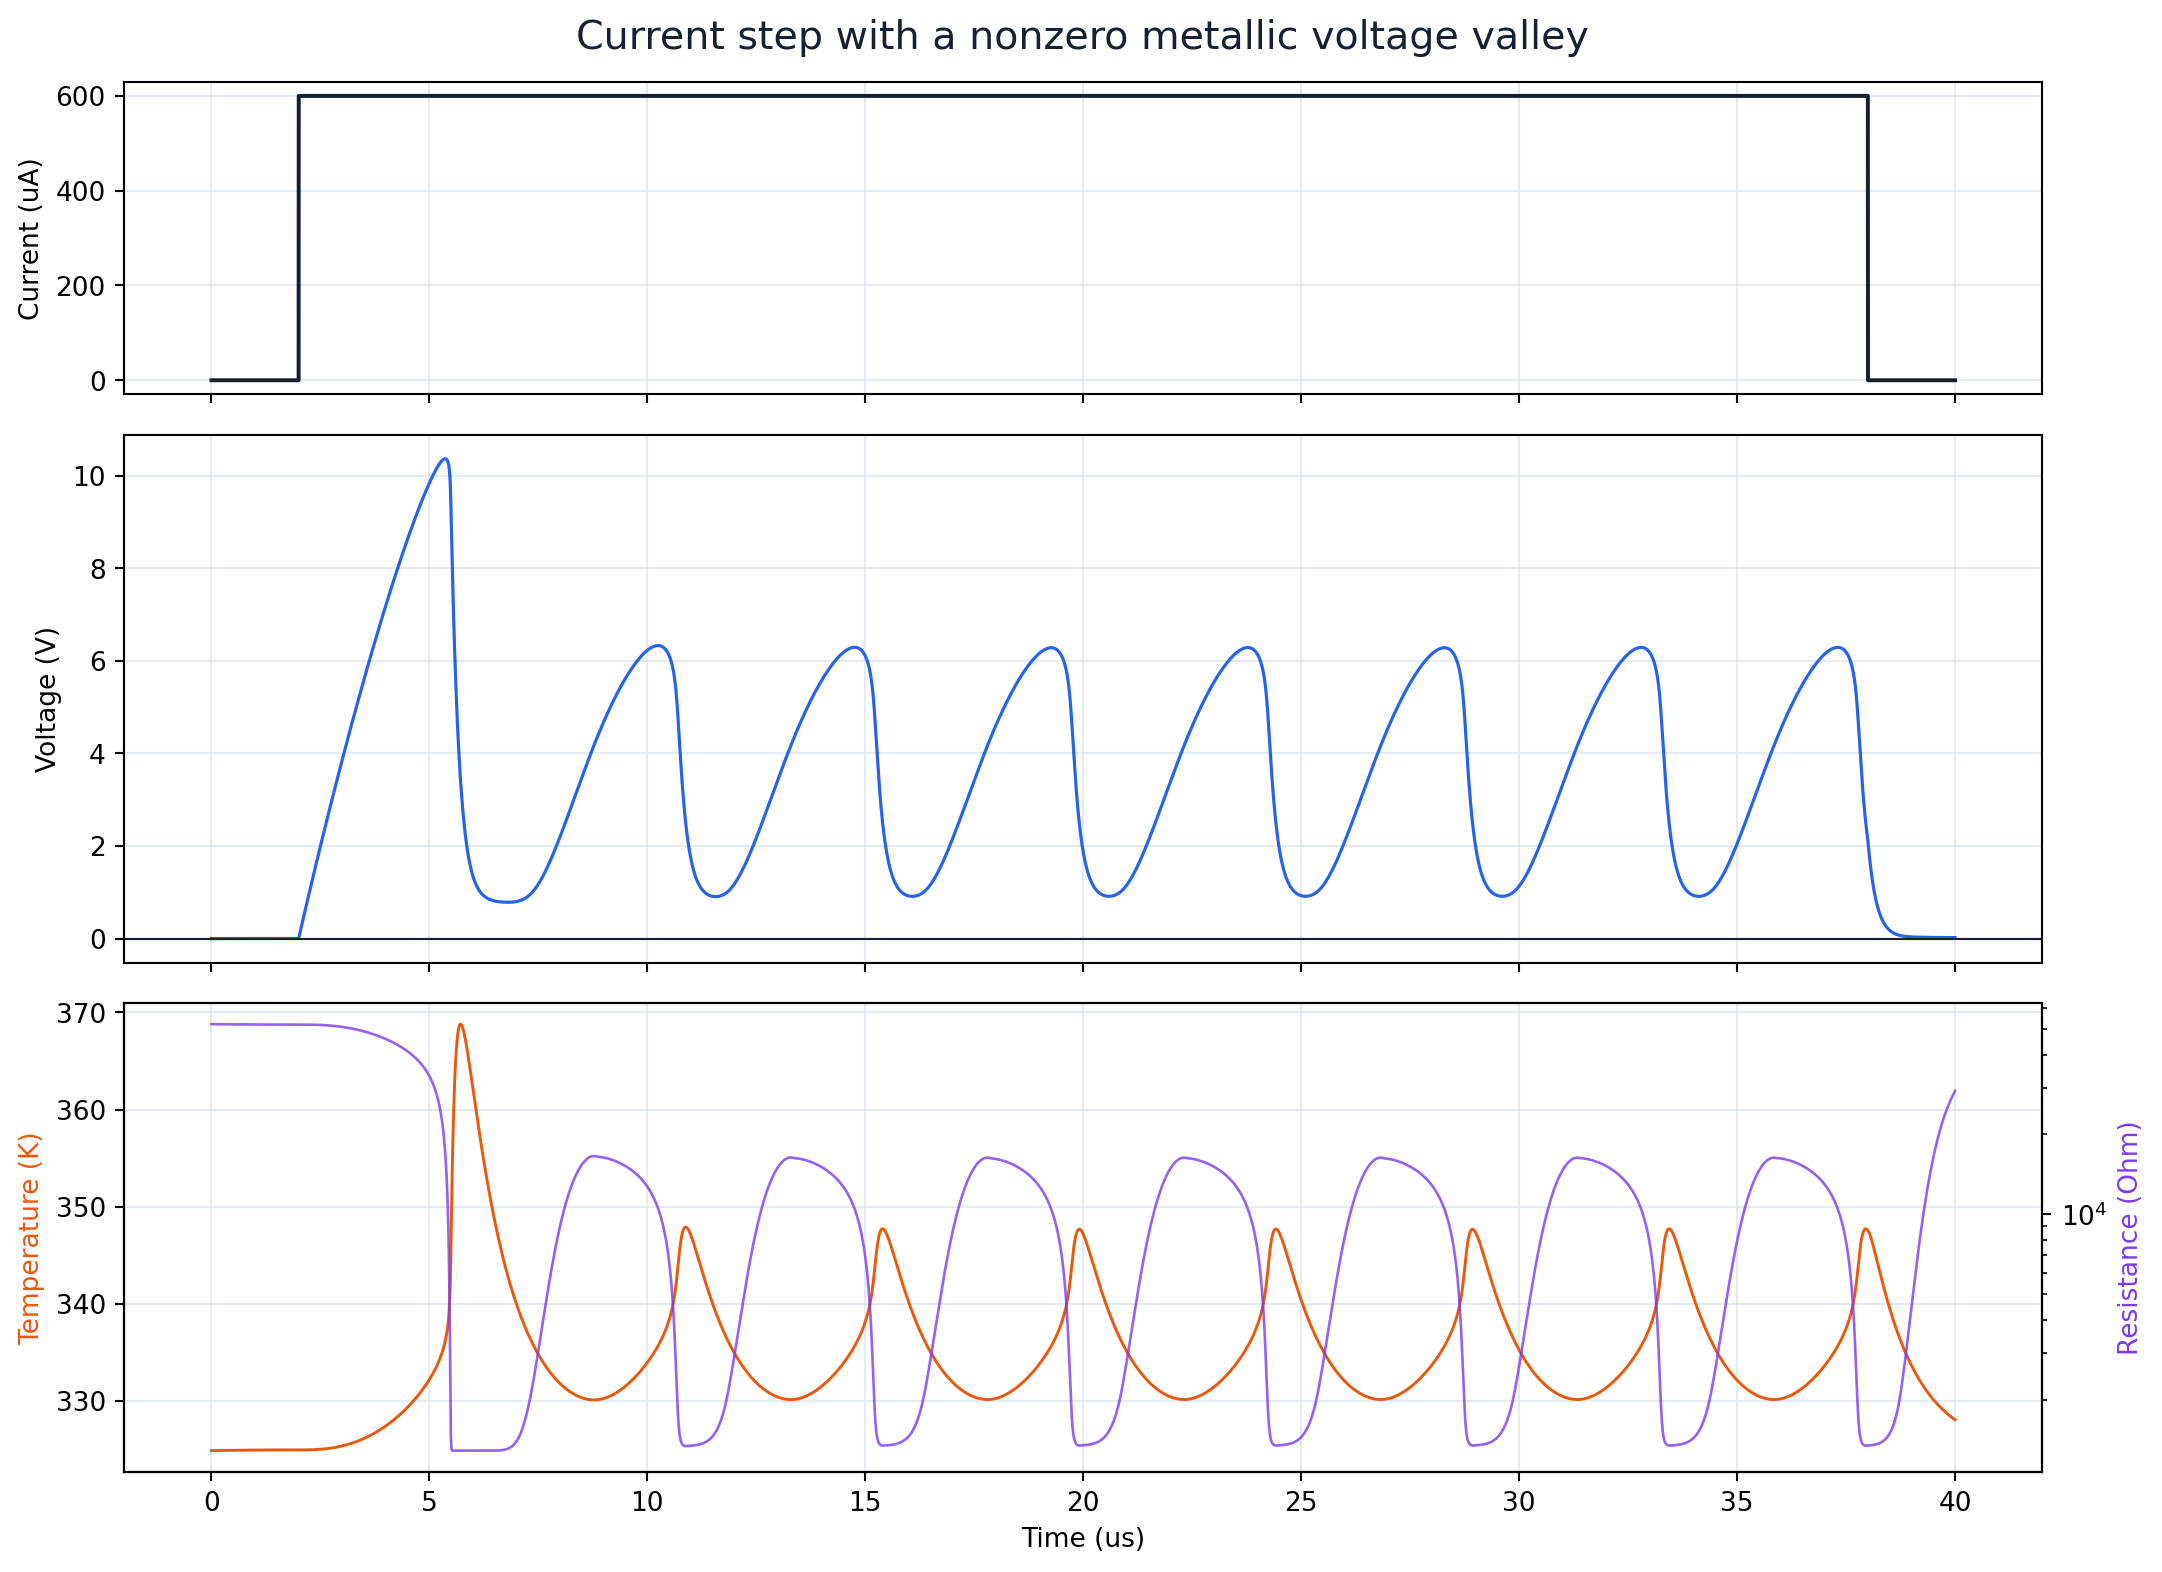
\includegraphics[width=\textwidth]{../../public_jobs/20260810_170502_current-step-with-a-nonzero-metallic-voltage-val_b05d39/figures/overview.png}
\caption{Applied current and simulated voltage, temperature, and resistance. The analysis excludes the initial charging transient and uses the stable interval from $10$ to $38~\mu$s.}
\label{fig:current_control}
\end{figure}

\begin{figure}[H]
\centering
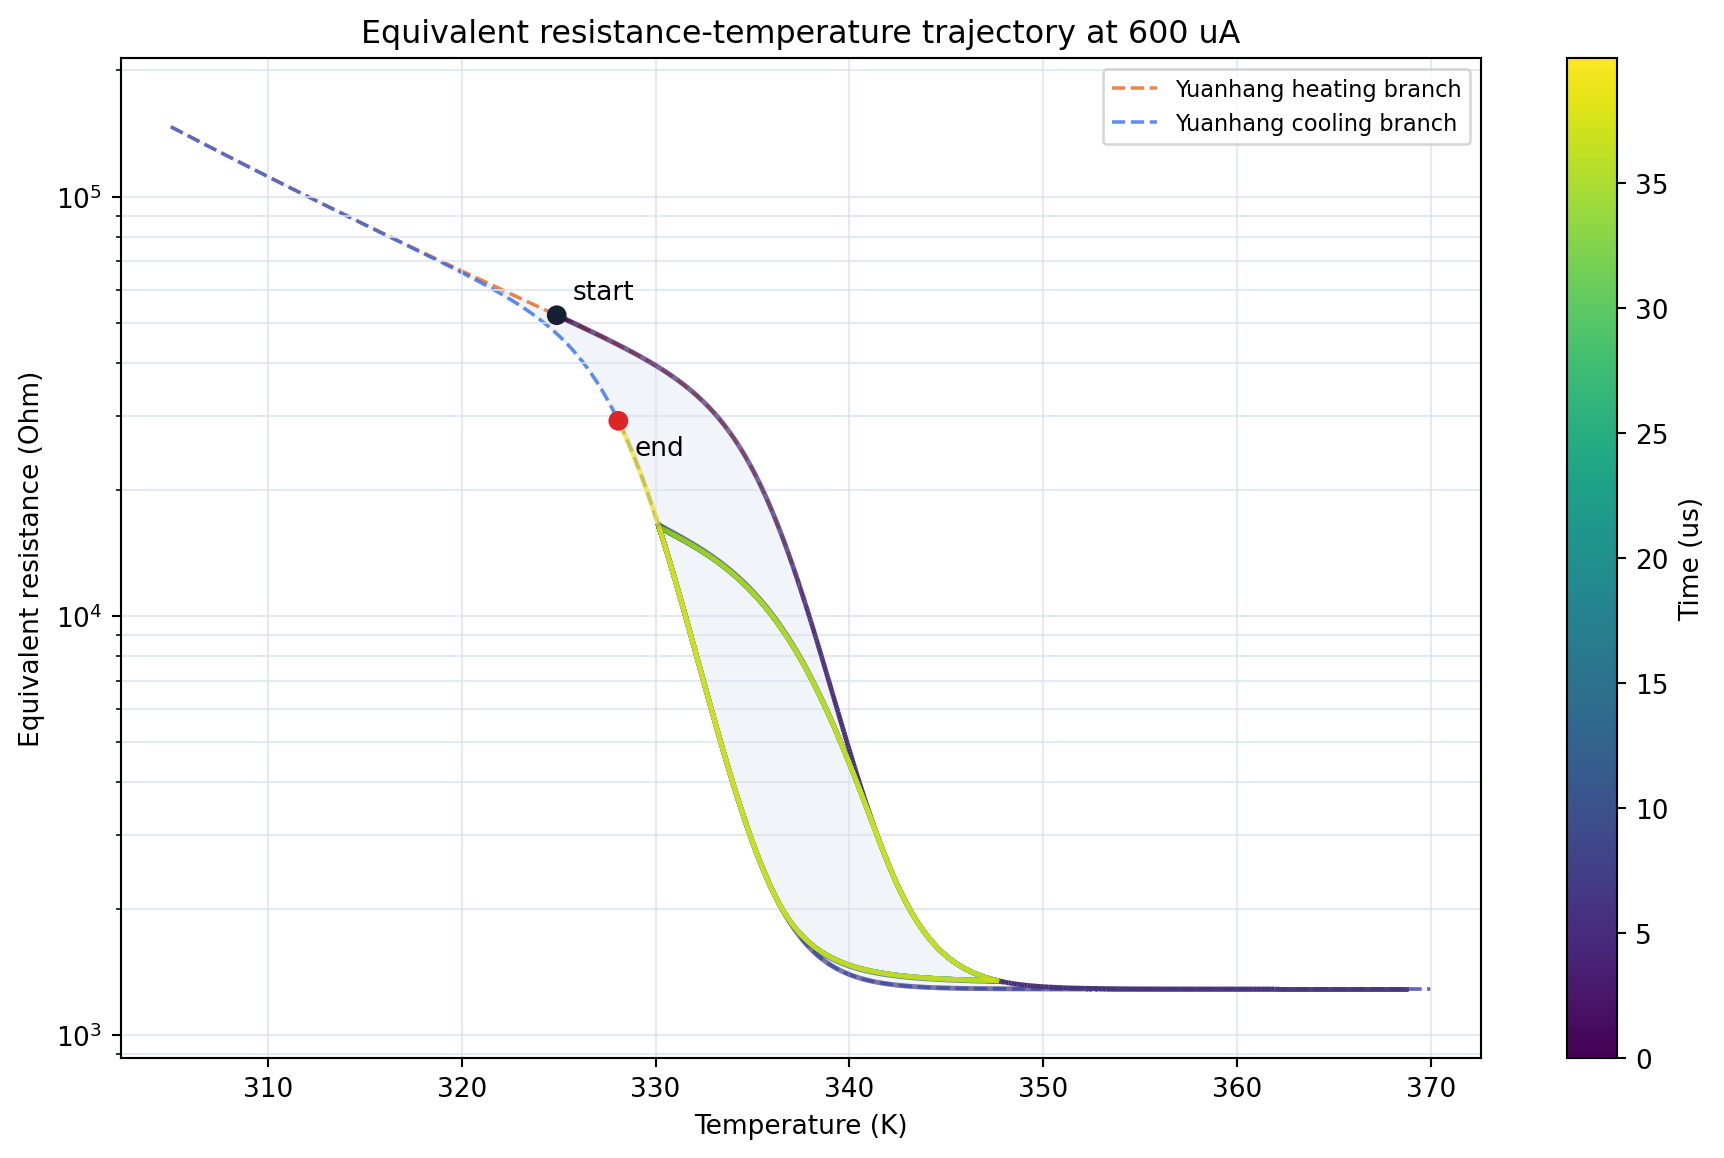
\includegraphics[width=0.88\textwidth]{figures/resistance_temperature_trajectory.png}
\caption{Equivalent resistance versus temperature. The dashed curves and shaded band show Yuanhang's major heating and cooling hysteresis; color shows progression through the $40~\mu$s simulated trajectory.}
\label{fig:rt_trajectory}
\end{figure}

\begin{table}[H]
\centering
\small
\rowcolors{2}{projectgray}{white}
\begin{tabular}{@{}l r@{}}
\toprule
Metric & Result \\
\midrule
Oscillation detected & yes \\
Detected cycles & 5 \\
Frequency & $0.221685$ MHz \\
Period & $4.51090~\mu$s \\
Period coefficient of variation & $1.77\times10^{-4}$ \\
Steady voltage range & $0.905654$--$6.33281$ V \\
Full-pulse temperature range & $324.9$--$368.8$ K \\
Steady temperature range & $330.16$--$347.91$ K \\
Steady resistance range & $1.339$--$16.382$ k$\Omega$ \\
Metallic electrical time $C R_m$ & $186.961$ ns \\
Thermal time $C_{\mathrm{th}}/S_e$ & $0.965581~\mu$s \\
\bottomrule
\end{tabular}
\caption{Metrics measured from the validation run.}
\label{tab:validation_results}
\end{table}

The metallic-state voltage is set approximately by $V=IR_m$:

\begin{equation}
V_{\mathrm{metal}}\approx I R_m
=(600\times10^{-6}\ \mathrm{A})(1286.3165\ \Omega)
=0.771790\ \mathrm{V}.
\label{eq:metal_floor}
\end{equation}

The simulated minimum is $0.905654$~V; it remains above this fixed point because switching reverses before the capacitor settles. The experimental manuscript reports $40$--$60$~MHz oscillations \cite{gildor2026}, whereas this validation gives $0.221685$~MHz. Sample-specific resistance and time constants are therefore still required for a quantitative match.

\section{Sample-specific resistance--temperature fit}

The supplied file contains 264 measurements from one cooling sweep and one heating sweep over $289.85$--$370.16$~K at $2~\mu$A. We fitted the major-loop form

\begin{equation}
R(T,\delta)=R_m+R_0 e^{(E_a/k_B)/T}
\left[\frac{1}{2}+\frac{1}{2}\tanh\!\left(\beta\left(\delta\frac{w}{2}+T_c-T\right)\right)\right],
\qquad
\delta=\begin{cases}-1,&\text{cooling},\\+1,&\text{heating}.
\end{cases}
\label{eq:sample_rt_fit}
\end{equation}

The fit minimizes the residual in $\log_{10}R$. Confidence intervals use 1000 circular block-bootstrap samples with eight-point blocks. The minor-loop parameter $\gamma$ was fixed to Yuanhang's value because a major loop alone does not determine it.

\begin{figure}[H]
\centering
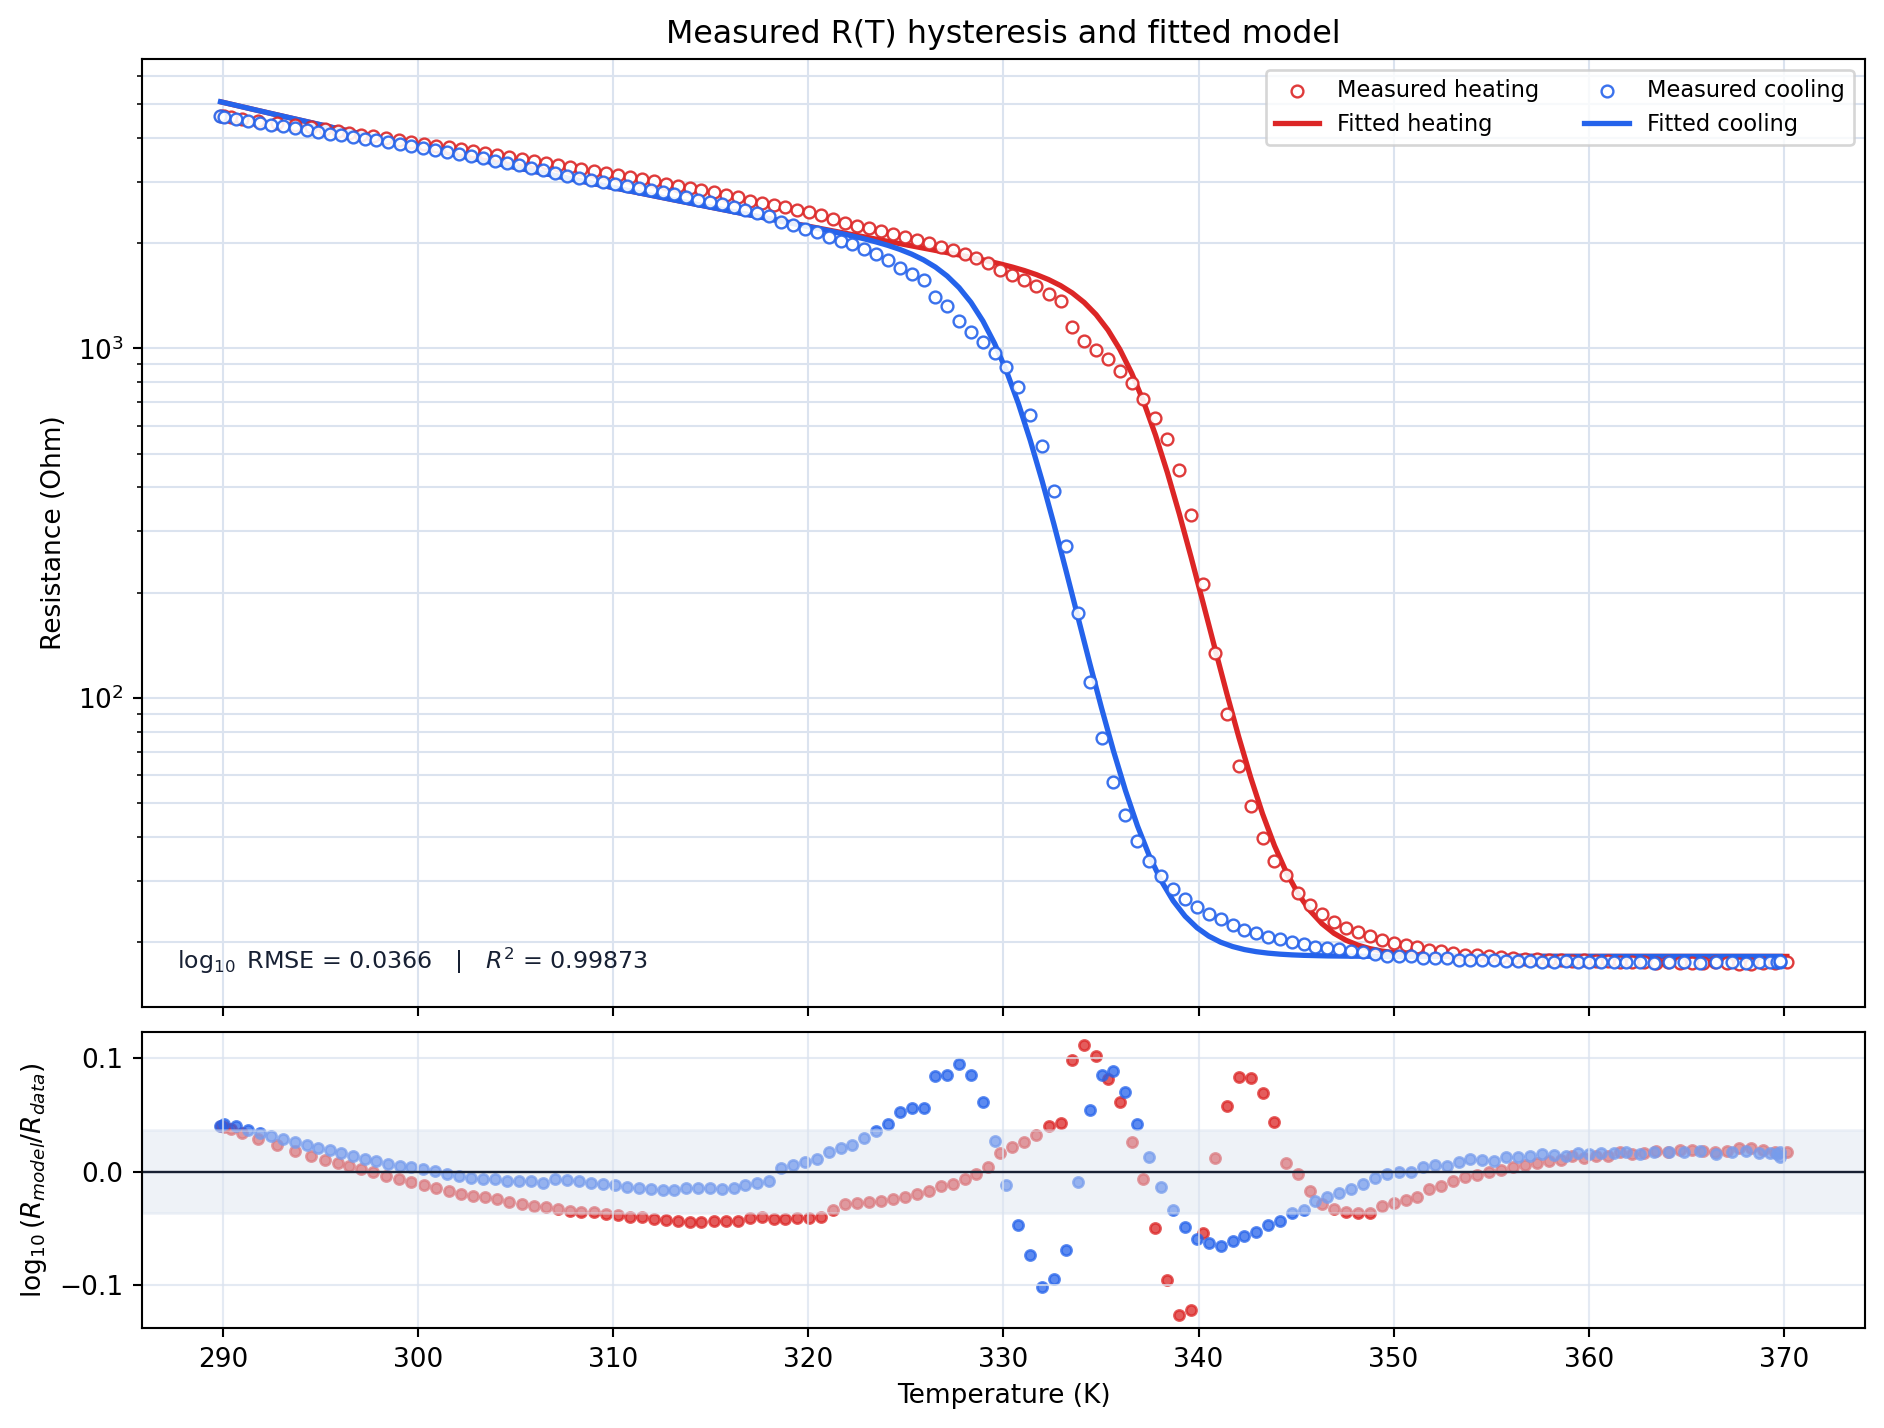
\includegraphics[width=0.96\textwidth]{../../public_jobs/20260816_125905_sample-r-t-major-loop-hysteresis-fit_0849a9/figures/resistance_fit.png}
\caption{Measured heating and cooling branches, fitted model, and log-resistance residuals.}
\label{fig:sample_rt_fit}
\end{figure}

\begin{table}[H]
\centering
\small
\rowcolors{2}{projectgray}{white}
\begin{tabular}{@{}l r r@{}}
\toprule
Parameter & Estimate & 95\% interval \\
\midrule
$R_0$ & $0.7989~\Omega$ & $0.3774$--$1.8483~\Omega$ \\
$E_a/k_B$ & $2536.97$ K & $2272.55$--$2767.52$ K \\
$E_a$ & $0.21862$ eV & $0.19583$--$0.23849$ eV \\
$R_m$ & $18.2153~\Omega$ & $17.4943$--$18.9010~\Omega$ \\
$T_c$ & $333.494$ K & $333.137$--$333.838$ K \\
$w$ & $6.8823$ K & $6.6291$--$7.2681$ K \\
$\beta$ & $0.29916~\mathrm{K}^{-1}$ & $0.28092$--$0.32021~\mathrm{K}^{-1}$ \\
$T_{\mathrm{cool}}=T_c-w/2$ & $330.052$ K & $329.642$--$330.385$ K \\
$T_{\mathrm{heat}}=T_c+w/2$ & $336.935$ K & $336.534$--$337.348$ K \\
$\gamma$ & $0.95627$ (fixed) & --- \\
\bottomrule
\end{tabular}
\caption{Sample-specific resistance parameters. $R_0$ and $E_a/k_B$ are strongly correlated; their joint combination, rather than either value alone, determines the insulating branch.}
\label{tab:sample_rt_parameters}
\end{table}

The fit gives $R^2=0.998734$ and a $\log_{10}R$ RMSE of $0.03663$, equivalent to a typical multiplicative error of $1.088$. The largest deviation is a factor of $1.336$ inside the switching region; this residual is retained rather than adding parameters unsupported by the measurement.

\section{Experimental conditions and measured operating points}

\planned{} Record the ambient temperature and exact current for every waveform. Extract the pre-switch voltage and current, switching direction, period, and voltage slopes. The switching power is

\begin{equation}
P_{\mathrm{sw}}=I_{\mathrm{sw}}V_{\mathrm{sw}}
=\frac{V_{\mathrm{sw}}^2}{R(T_{\mathrm{sw}})}.
\end{equation}

Together with the fitted $R(T)$ transition temperatures, these measurements provide the remaining inputs.

\section{Environmental thermal conductance}

\planned{} At a verified quasi-steady point, use the relevant heating or cooling transition temperature to estimate

\begin{equation}
S_e=\frac{P_{\mathrm{sw}}}{T_{\mathrm{sw}}-T_0},
\qquad
\left.\frac{dT}{dt}\right|_{\mathrm{sw}}\approx0.
\end{equation}

The selected point, voltage definition, and quasi-steady assumption will be stated explicitly; agreement across currents will test consistency.

\newpage
\thispagestyle{fancy}
\section{Electrical capacitance}

\planned{} Determine the effective capacitance from a nonswitching transient, separating electrical charging from the later thermal response. At the beginning of a current step, where $V/R(T)\ll I$, the current-balance estimate below reduces to $C\approx I/(dV/dt)$:

\begin{equation}
C=\frac{\tau_{\mathrm{el}}}{R_{\mathrm{eff}}}
\qquad\text{or}\qquad
C=\frac{I-V/R(T)}{dV/dt}.
\end{equation}

\section{Thermal time constant and thermal capacitance}

\planned{} With $R(T)$, $T_0$, $S_e$, and $C$ fixed, fit the measured thermal relaxation or switching interval to obtain $\tau_{\mathrm{th}}$, then calculate

\begin{equation}
C_{\mathrm{th}}=S_e\tau_{\mathrm{th}}.
\end{equation}

An independent geometry estimate, $C_{\mathrm{th}}=\rho c_p V$, will be used as a cross-check rather than as the primary dynamical estimate. Assumed active volume and material values will be reported with their uncertainty.

\section{Comparison across experimental currents}

\planned{} Simulate the measured current amplitudes without per-trace retuning. Compare oscillation onset and cessation, frequency, voltage extrema, average voltage, and energy per cycle using common axes.

\section{Capacitance dependence and the thermal-only limit}

\planned{} Map oscillation frequency over $C$ and $C_{\mathrm{th}}$ for each current. The zero-capacitance limit will be evaluated using

\begin{equation}
C=0 \quad\Longrightarrow\quad V(t)=I_{\mathrm{in}}(t)R(T),
\qquad
\tau_{\mathrm{th}}=\frac{C_{\mathrm{th}}}{S_e}.
\end{equation}

\appendix
\section{Reproduction}

The validation run is archived as

\begin{center}
\footnotesize
\path{20260810_170502_current-step-with-a-nonzero-metallic-voltage-val_b05d39}.
\end{center}

It can be reproduced from the repository root with

\begin{center}
\ttfamily\small
neuristor simulate current --config experiments/current/nonzero\_voltage\_valley.toml
\end{center}

The archived bundle contains the resolved configuration, traces, metrics, figure, and repository provenance. A fresh execution produced identical metrics and byte-identical trace data.

The resistance--temperature figure and synchronized GIF are regenerated from the same archived traces with \texttt{neuristor runs visualize}.

The sample resistance fit is archived as

\begin{center}
\footnotesize
\path{20260816_125905_sample-r-t-major-loop-hysteresis-fit_0849a9}.
\end{center}

It is reproduced with

\begin{center}
\ttfamily\small
neuristor fit resistance --data data/experimental/100425\_chip1\_gap3.tsv --method major-loop --bootstrap-samples 1000
\end{center}

\begin{thebibliography}{9}

\bibitem{zhang2024}
Y.-H. Zhang, C. Sipling, E. Qiu, I. K. Schuller, and M. Di Ventra,
``Collective dynamics and long-range order in thermal neuristor networks,''
\emph{Nature Communications}, vol. 15, art. 6986, 2024.
\href{https://doi.org/10.1038/s41467-024-51254-4}{doi:10.1038/s41467-024-51254-4}.

\bibitem{gildor2026}
A. Gildor, S. Hodisan, S. Kvatinsky, and Y. Kalcheim,
``Harnessing the \vo{} Phase Transition for Automatic Gain Control in Transimpedance Amplifiers,''
manuscript, arXiv:2604.04594v1, 2026.

\end{thebibliography}

\end{document}
